\beginsong{Nachts auf dem Dorfplatz}[
    wuw={Turi (Kurt Kremers)},
    jahr={1964}, 
    bo={240},
    pfii={116}, 
    gruen={57}, 
    kssiv={24}, 
    siru={167}, 
    tonspur={406},
]

\beginverse
\endverse
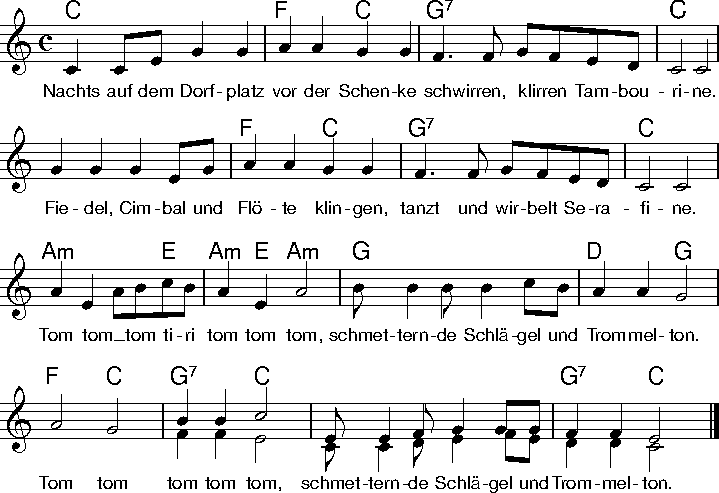
\includegraphics[draft=false, width=1\textwidth]{Noten/Lied067.pdf}

\beginverse
\[C]Her mit dem Weinkrug \[F]voll zum \[C]Rande, \[G7]trinkt zur Neige, durst'ge \[C]Zecher!
Zigan, spielst du die \[F]Sara\[C]bande, \[G]lockt als Lohn ein gold'ner \[C]Becher.
\endverse

\beginchorus
\[Am]Tom tom tom \[E]tiri \[Am]tom \[E]tom \[Am]tom, \[G]schmetternde Schlägel und \[D]Trommel\[G]ton:
\[F]Tom \[C]tom \[G7]tom tom \[C]tom, schmetternde Schlägel und \[G7]Trommel\[C]ton.
\endchorus
 
\beginverse
^Knöcherne Finger ^alter ^Fetteln ^lesen Zukunft aus den ^Händen,
Pfeife rauchend und ^Tabak ^bettelnd, ^dürre Beine, feiste ^Lenden.
\endverse

\beginchorus
\[Am]Tom tom tom \[E]tiri \[Am]tom \[E]tom \[Am]tom, \[G]schmetternde Schlägel und \[D]Trommel\[G]ton:
\[F]Tom \[C]tom \[G7]tom tom \[C]tom, schmetternde Schlägel und \[G7]Trommel\[C]ton.
\endchorus

\beginverse
^Segelt des Mondes ^stille ^Barke ^über Pinien und Pla^tanen.
Mitternacht wird zur ^Wende^marke, ^lässt den jungen Tag schon ^ahnen.
\endverse

\beginchorus
\[Am]Tom tom tom \[E]tiri \[Am]tom \[E]tom \[Am]tom, \[G]leis' werden Schlägel und \[D]Trommel\[G]ton:
\lrep \[F]Tom \[C]tom \[G7]tom tom \[C]tom, leis' werden Schlägel und \[G7]Trommel\[C]ton.\rrep
\endchorus

\endsong

\beginscripture{}
Das Lied ist auch bekannt unter dem Titel~ ''Die Schenke von Novo Selo''.
\endscripture
